\documentclass[a4paper,11.5pt]{article}
\usepackage[textwidth=170mm, textheight=230mm, inner=20mm, top=20mm, bottom=30mm]{geometry}
\usepackage[normalem]{ulem}
\usepackage[utf8]{inputenc}
\usepackage[T1]{fontenc}
\PassOptionsToPackage{defaults=hu-min}{magyar.ldf}
\usepackage[magyar]{babel}
\usepackage{amsmath, amsthm,amssymb,paralist,array, ellipsis, graphicx,float}
%\usepackage{marvosym}

\makeatletter
\renewcommand*{\mathellipsis}{%
	\mathinner{%
		\kern\ellipsisbeforegap%
		{\ldotp}\kern\ellipsisgap%
		{\ldotp}\kern\ellipsisgap%
		{\ldotp}\kern\ellipsisaftergap%
	}%
}
\renewcommand*{\dotsb@}{%
	\mathinner{%
		\kern\ellipsisbeforegap%
		{\cdotp}\kern\ellipsisgap%
		{\cdotp}\kern\ellipsisgap%
		{\cdotp}\kern\ellipsisaftergap%
	}%
}
\renewcommand*{\@cdots}{%
	\mathinner{%
		\kern\ellipsisbeforegap%
		{\cdotp}\kern\ellipsisgap%
		{\cdotp}\kern\ellipsisgap%
		{\cdotp}\kern\ellipsisaftergap%
	}%
}
\renewcommand*{\ellipsis@default}{%
	\ellipsis@before
	\kern\ellipsisbeforegap
	.\kern\ellipsisgap
	.\kern\ellipsisgap
	.\kern\ellipsisgap
	\ellipsis@after\relax}
\renewcommand*{\ellipsis@centered}{%
	\ellipsis@before
	\kern\ellipsisbeforegap
	.\kern\ellipsisgap
	.\kern\ellipsisgap
	.\kern\ellipsisaftergap
	\ellipsis@after\relax}
\AtBeginDocument{%
	\DeclareRobustCommand*{\dots}{%
		\ifmmode\@xp\mdots@\else\@xp\textellipsis\fi}}
\def\ellipsisgap{.1em}
\def\ellipsisbeforegap{.05em}
\def\ellipsisaftergap{.05em}
\makeatother

\usepackage{hyperref}
\hypersetup{
	colorlinks = true	
}

\begin{document}
	%%%%%%%%%%%RÖVIDÍTÉSEK%%%%%%%%%%
	\setlength\parindent{0pt}
	\def\s{\hspace{0.2mm}\vphantom{\beta}}
	\def\Z{\mathbb{Z}}
	\def\Q{\mathbb{Q}}
	\def\R{\mathbb{R}}
	\def\C{\mathbb{C}}
	\def\N{\mathbb{N}}
	\def\Ra{\overline{\mathbb{R}}}
	
	\def\sume{\displaystyle\sum_{n=1}^{+\infty}}
	\def\sumn{\displaystyle\sum_{n=0}^{+\infty}}
	
	\def\narrow{\underset{n\rightarrow+\infty}{\longrightarrow}}
	\def\limn{\displaystyle\lim_{n\to +\infty}}
	\def\limx{\displaystyle\lim_{x\to +\infty}}
	
	\theoremstyle{definition}
	\newtheorem{theorem}{Tétel}[subsection] 
	
	\theoremstyle{definition}
	\newtheorem{definition}[theorem]{Definíció} 
	\newtheorem{example}[theorem]{Példa} 
	\newtheorem{task}[theorem]{Feladat} 
	\newtheorem{note}[theorem]{Megjegyzés}
	\newtheorem{revision}[theorem]{Emlékeztető}
	%%%%%%%%%%%%%%%%%%%%%%%%%%%%%%%%%%%%%%%%%%%%%%%%%%%%%%%%%%%%%%%%%%%%%
	\begin{center}
		{\LARGE\textbf{Analízis II.}}
		
		{\Large Előadás jegyzet}
		
		3. óra.
	\end{center}
	A jegyzetet \textsc{Umann} Kristóf készítette Dr. \textsc{Szili} László  előadásán. (\today)
	
	Külön köszönet jár \textsc{Csonka} Szilviának a képek elkészítésért.
	\bigskip
	
	Tantárgyi honlap: \url{http://numanal.inf.elte.hu/~szili/Oktatas/An2_BSc_2016/index_An2_2016.htm}
	
	\section{Folytatás.}
	\begin{revision}
		Szakadási helyek, osztályozás.
		\begin{example}\
			
			\begin{figure}[H]
				\centering
				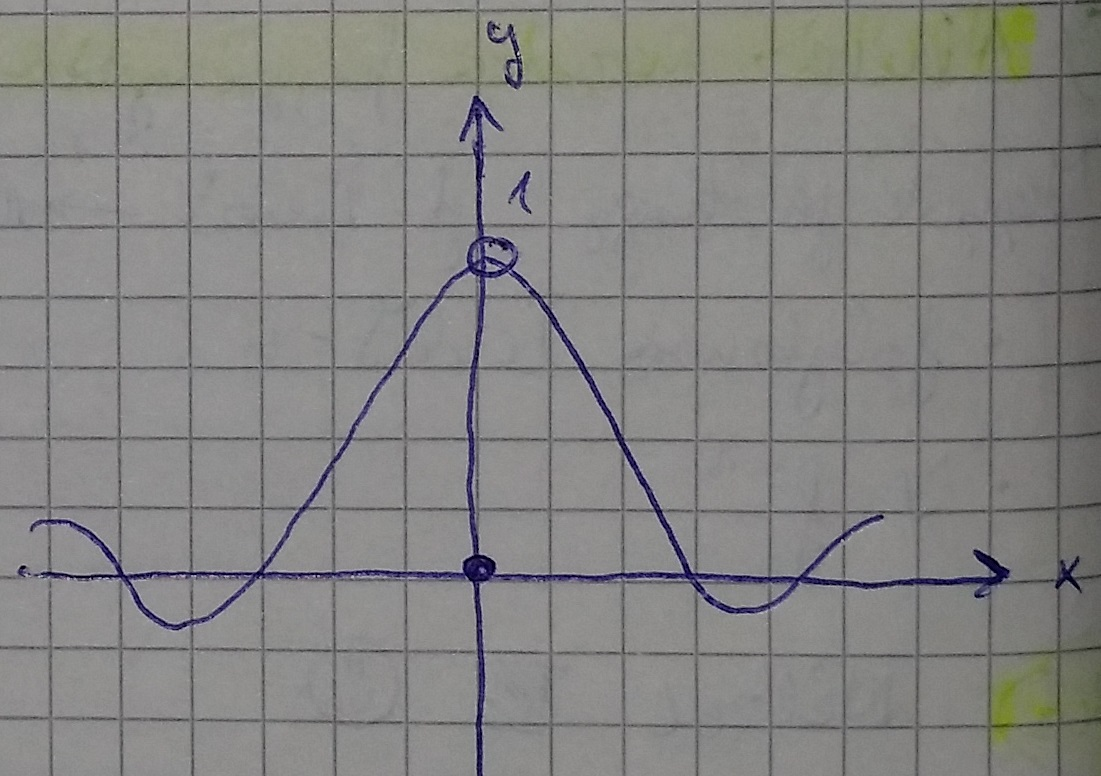
\includegraphics[height=3cm]{kepek/03ea_1.jpg}
				\caption{}\label{}
			\end{figure}
			\[ f(x) = \left\{\begin{gathered}
			\frac{\sin(x)}{x}, \quad x\in\R\setminus\{0\}\\
			0, \quad x=0
			\end{gathered}\right.\]
			Ezalapján megállapítható:
			\begin{enumerate}
				\item $f\in C\{a\}, \quad \forall a \not=0$
				\item $a=0$ megszüntethető szakadási hely, mert $\displaystyle \lim_{x\to0}\frac{\sin(x)}{x} = 0 \not=f(0)=0.$
			\end{enumerate}
			Ha 
			\[ \tilde{f}(x) = \left\{\begin{gathered}
			f(x), \quad x\in\R\setminus\{0\}\\
			1, \quad x=0
			\end{gathered}\right. \]
			akkor $\tilde{f}\in C\{0\}$.
			
		\end{example}
		\begin{example}
			\[ f(x):=\text{sign}(x)\quad (x\in\R) \]
			
			\begin{figure}[H]
				\centering
				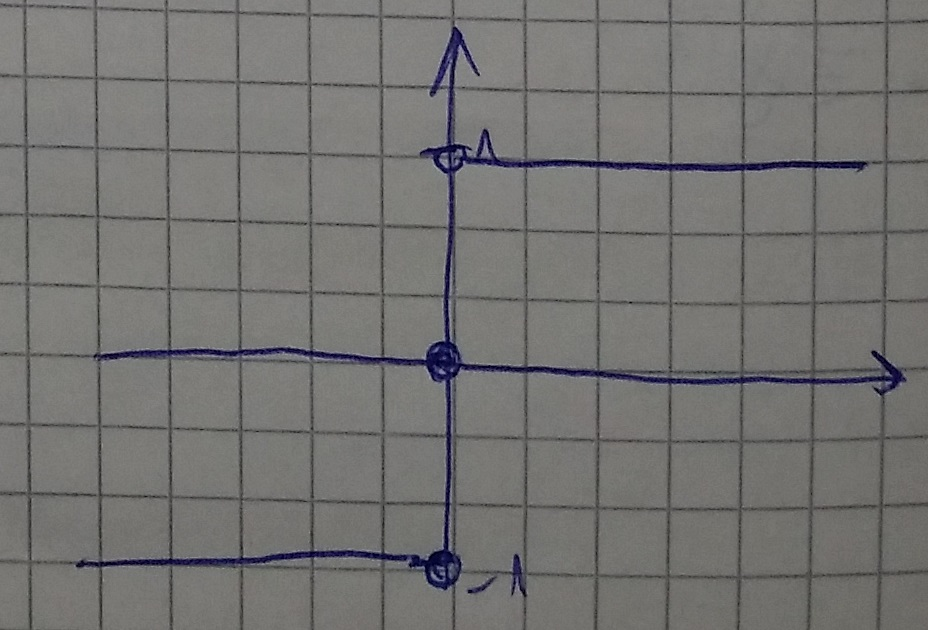
\includegraphics[height=3cm]{kepek/03ea_2.jpg}
				\caption{}\label{}
			\end{figure}
			\begin{enumerate}
				\item $f\in C\{a\}, \quad \forall a\in\R\setminus\{0\}$
				\item az $a=0$ elsőfajú szakadási hely, mert \quad $\displaystyle \exists \lim_{0+0}f=1\not=\exists\lim_{0-0}f=-1$.
			\end{enumerate}
		\end{example}
		\begin{note}
			Másodfajú szakadás sokféleképpen lehet.
			\begin{example}
				Dirichlet-fv.
				\[ f(x)=\left\{\begin{gathered}
				1,\quad x\in\Q\\
				0,\quad x\in\Q^*
				\end{gathered}\right. \]
				\begin{figure}[H]
					\centering
					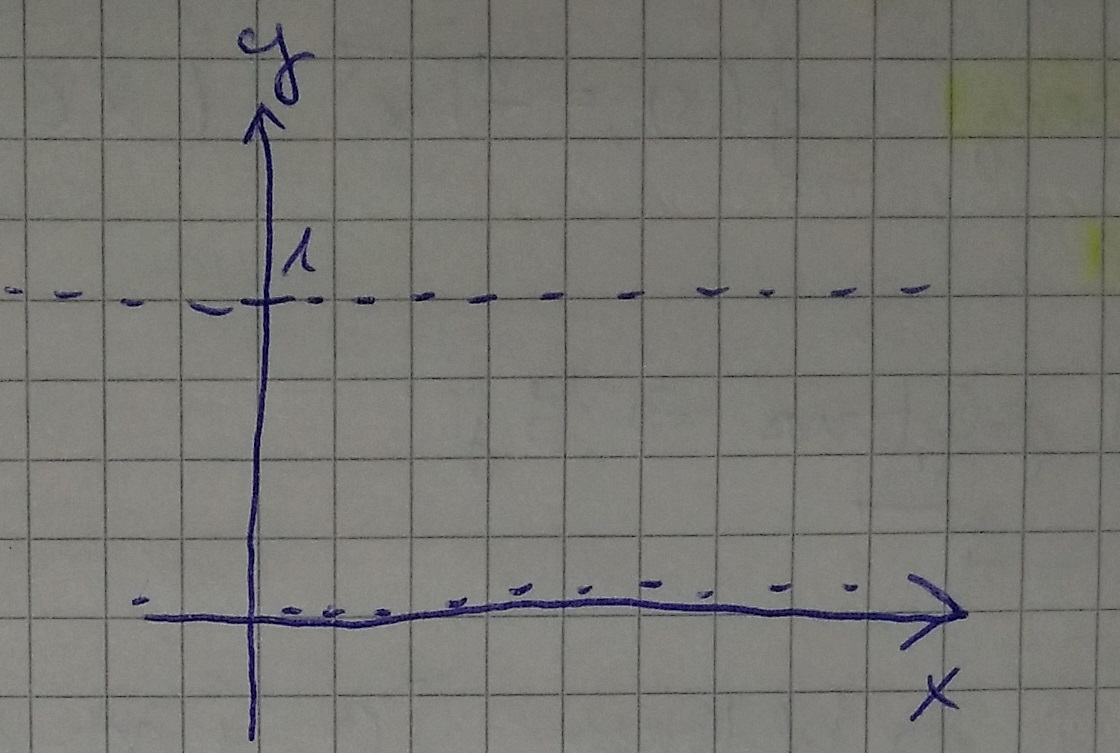
\includegraphics[height=3cm]{kepek/03ea_3.jpg}
					\caption{}\label{}
				\end{figure}
				$\forall a\in \R$ másodfajú szakadási hely, mert $\displaystyle \nexists\lim_{a+0}f,\lim_{a-0}f$.
			\end{example}
			\begin{example}
				Dirichlet típusú függvény.
				\[ f(x)=\left\{\begin{gathered}
				x,\quad x\in\Q\\
				0,\quad x\in\Q^*
				\end{gathered}\right. \]
				\begin{figure}[H]
					\centering
					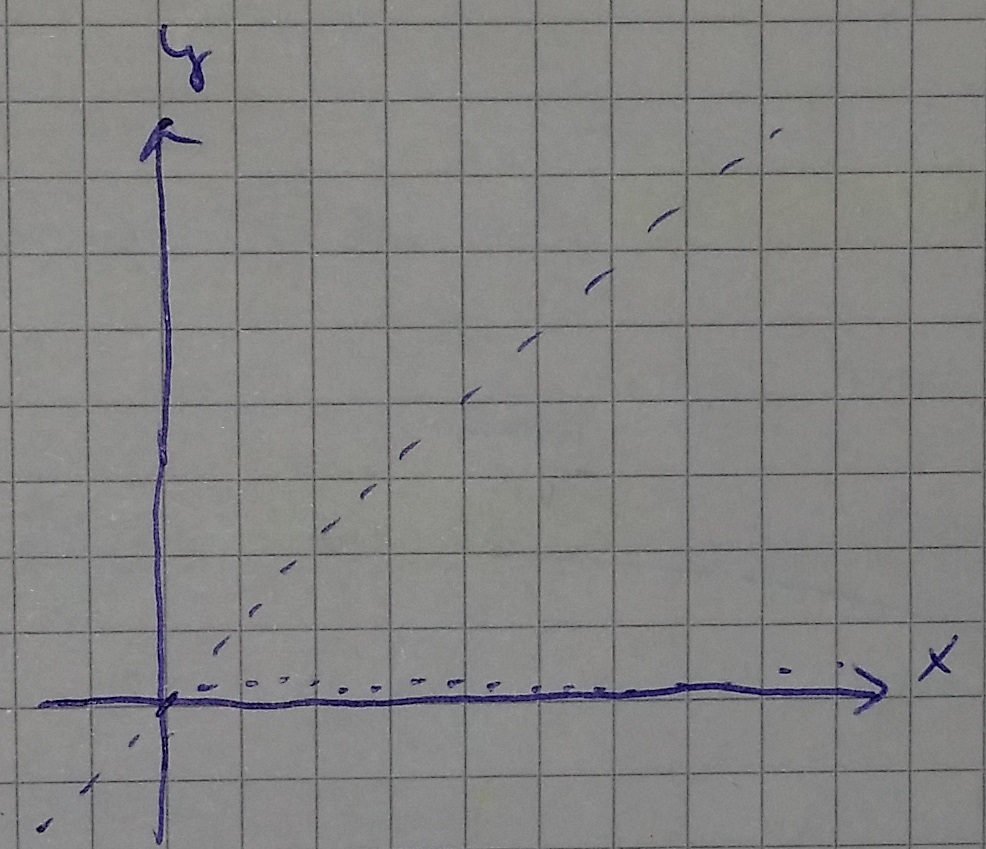
\includegraphics[height=3cm]{kepek/03ea_4.jpg}
					\caption{}\label{}
				\end{figure}
				\begin{enumerate}
					\item $f\in C\{0\}\checkmark$
					\item $\forall a\in\R\setminus\{0\}$ pont másodfajú szakadási hely.
				\end{enumerate}
			\end{example}
			\begin{example}
				\[ f(x)=\left\{\begin{gathered}
				\frac{1}{x}\quad x>0\\
				10,\quad x=0\\
				0,\quad x<0
				\end{gathered}\right. \]
				\begin{figure}[H]
					\centering
					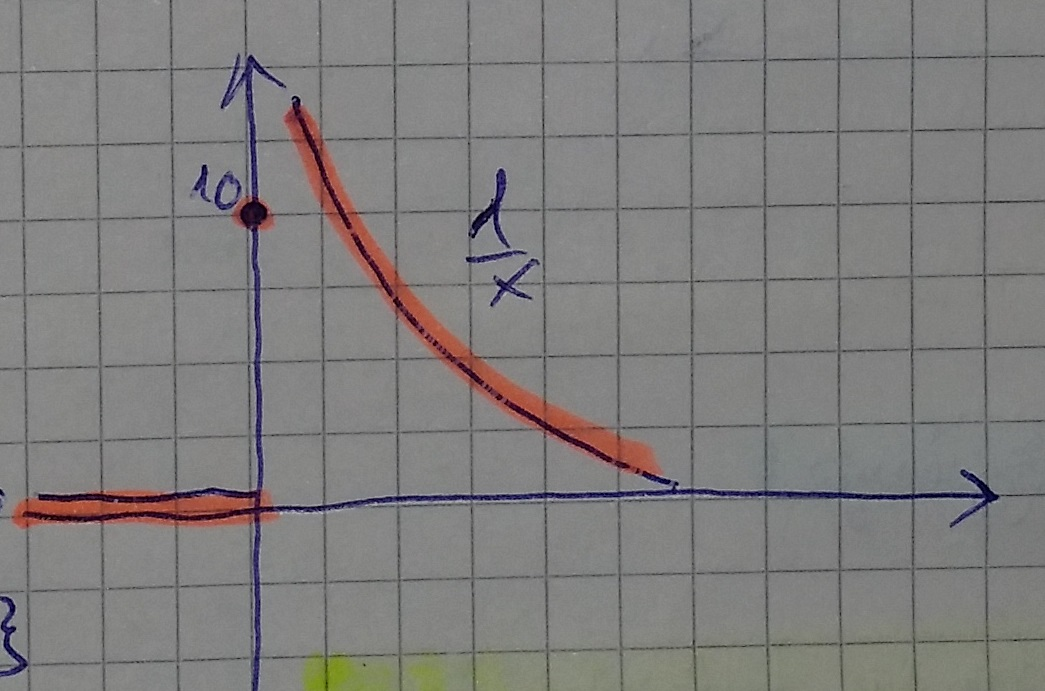
\includegraphics[height=3cm]{kepek/03ea_5.jpg}
					\caption{}\label{}
				\end{figure}
				\begin{enumerate}
					\item $f\in C\{a\}, \quad a\in \R\setminus\{0\}$
					\item $a=0$ másodfajú szakadási hely, mert $\lim_{x\to0+0}f(x)=\lim_{x\to0+0}\frac{1}{x}=+\infty$
				\end{enumerate}
			\end{example}
		\end{note}
	\end{revision}
	\begin{theorem}
		(Monoton függvény szakadási helyei)
		
		Ha $f:(\alpha,\beta)\to\R$ monoton függvény ($\alpha,\beta)$-n, akkor legfeljebb elsőfajú szakadásai lehetnek, azaz egy $a\in\mathcal{D}_f$ pontban az $f$ vagy folytonos, vagy elsőfajú szakadása van.
		
		\medskip
		\textit{biz nélkül.} 
	\end{theorem}
	\section{Elemi függvények.}
	\subsection{Hatvány- és gyökfüggvények.}
	\begin{revision}
		(hatványfüggvény)
		\quad \quad $f(x):=x^n\quad (x\in[0,+\infty))$
	\end{revision}
	\begin{revision}
		(gyökfüggvény)
		\quad \quad $f(x):=\sqrt[n]{x},\quad (x\in[0,+\infty))$
	\end{revision}
	Igazolható:
	\begin{itemize}
		\item $f \uparrow$ folytonos $\Rightarrow\exists f^{-1}$
		\item $\left|f^{-1}=\sqrt[n]{}\right|$
		\item $f^{-1}\uparrow$ és folytonos $[0,+\infty)$-n.
	\end{itemize}
	A függvények képe:
	
	\begin{figure}[H]
		\centering
		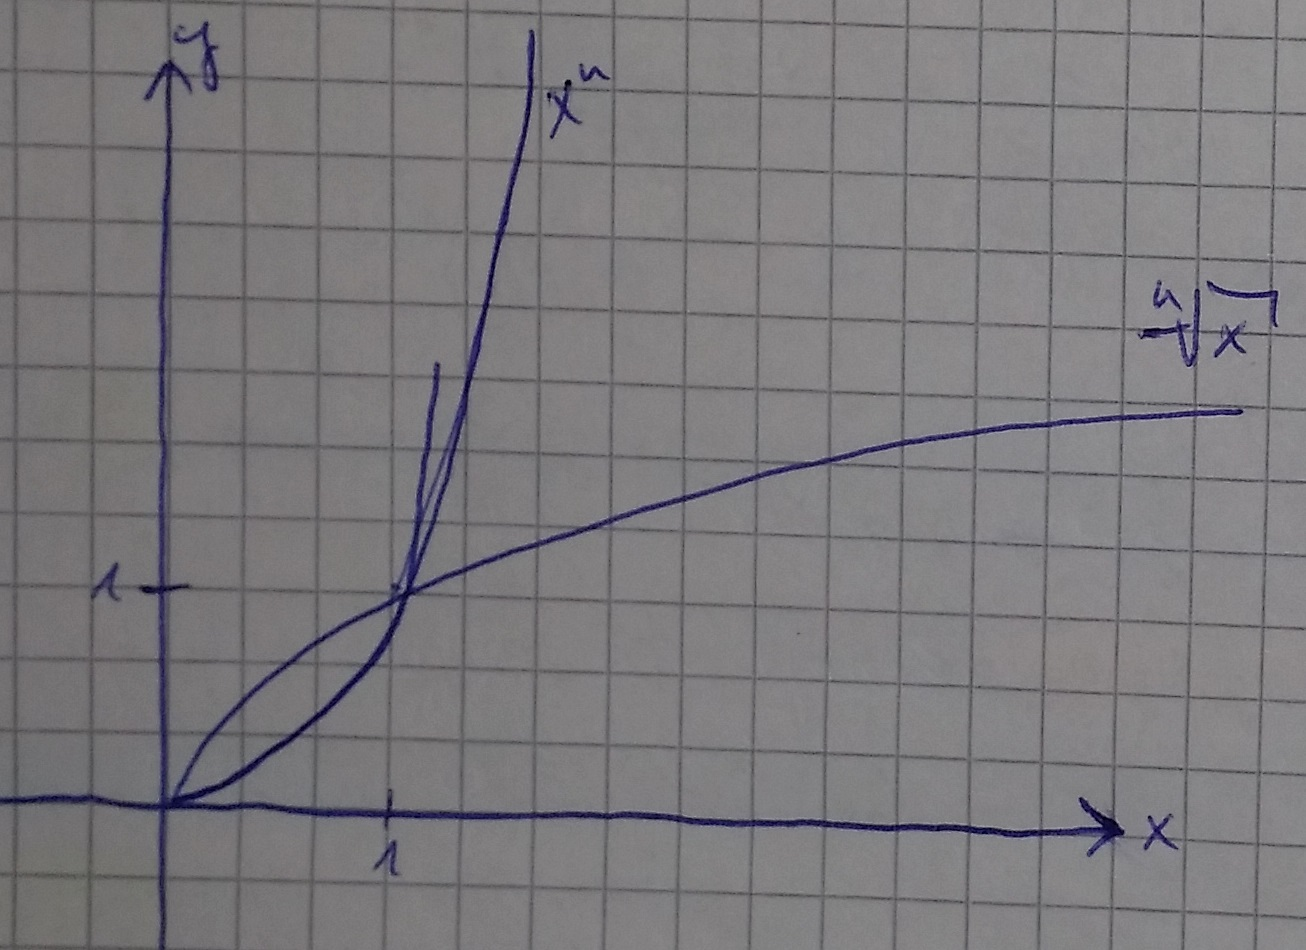
\includegraphics[height=3cm]{kepek/03ea_6.jpg}
		\caption{}\label{}
	\end{figure}
	\subsection{Az $\exp$ és az $\ln$ függvények.}
	\begin{theorem}
		(Az $\exp$ függvény tulajdonságai)
		
		\begin{enumerate}
			\item $\exp(x)\quad :=\quad \exp x\quad := \quad e^x\quad :=\quad \sumn\frac{x^n}{n!}\quad (x\in\R, \quad n\in\N)$
			\item (helyettesítési értékek)
			\begin{enumerate}
				\item $\exp(0)=1$
				\item $\exp(1)=\sumn\frac{1}{n!}=e\quad \left(\limn\left(1+\frac{1}{n}\right)^n \right)$
			\end{enumerate}
			\item A függvény egyenlet:
			$\quad \quad  e^{x+y}=e^x\cdot e^y\quad (x,y\in\R) $
			\item $\exp\uparrow$ folytonos $\R$-en.
			\item $\mathcal{R}_{\exp}=(0;+\infty)$.
			\item $\displaystyle \lim_{+\infty}\exp=+\infty,\quad \lim_{-\infty}\exp=0$.
		\end{enumerate}
		\medskip
		
		\textit{biz nélkül.}
	\end{theorem}
	
	\begin{figure}[H]
		\centering
		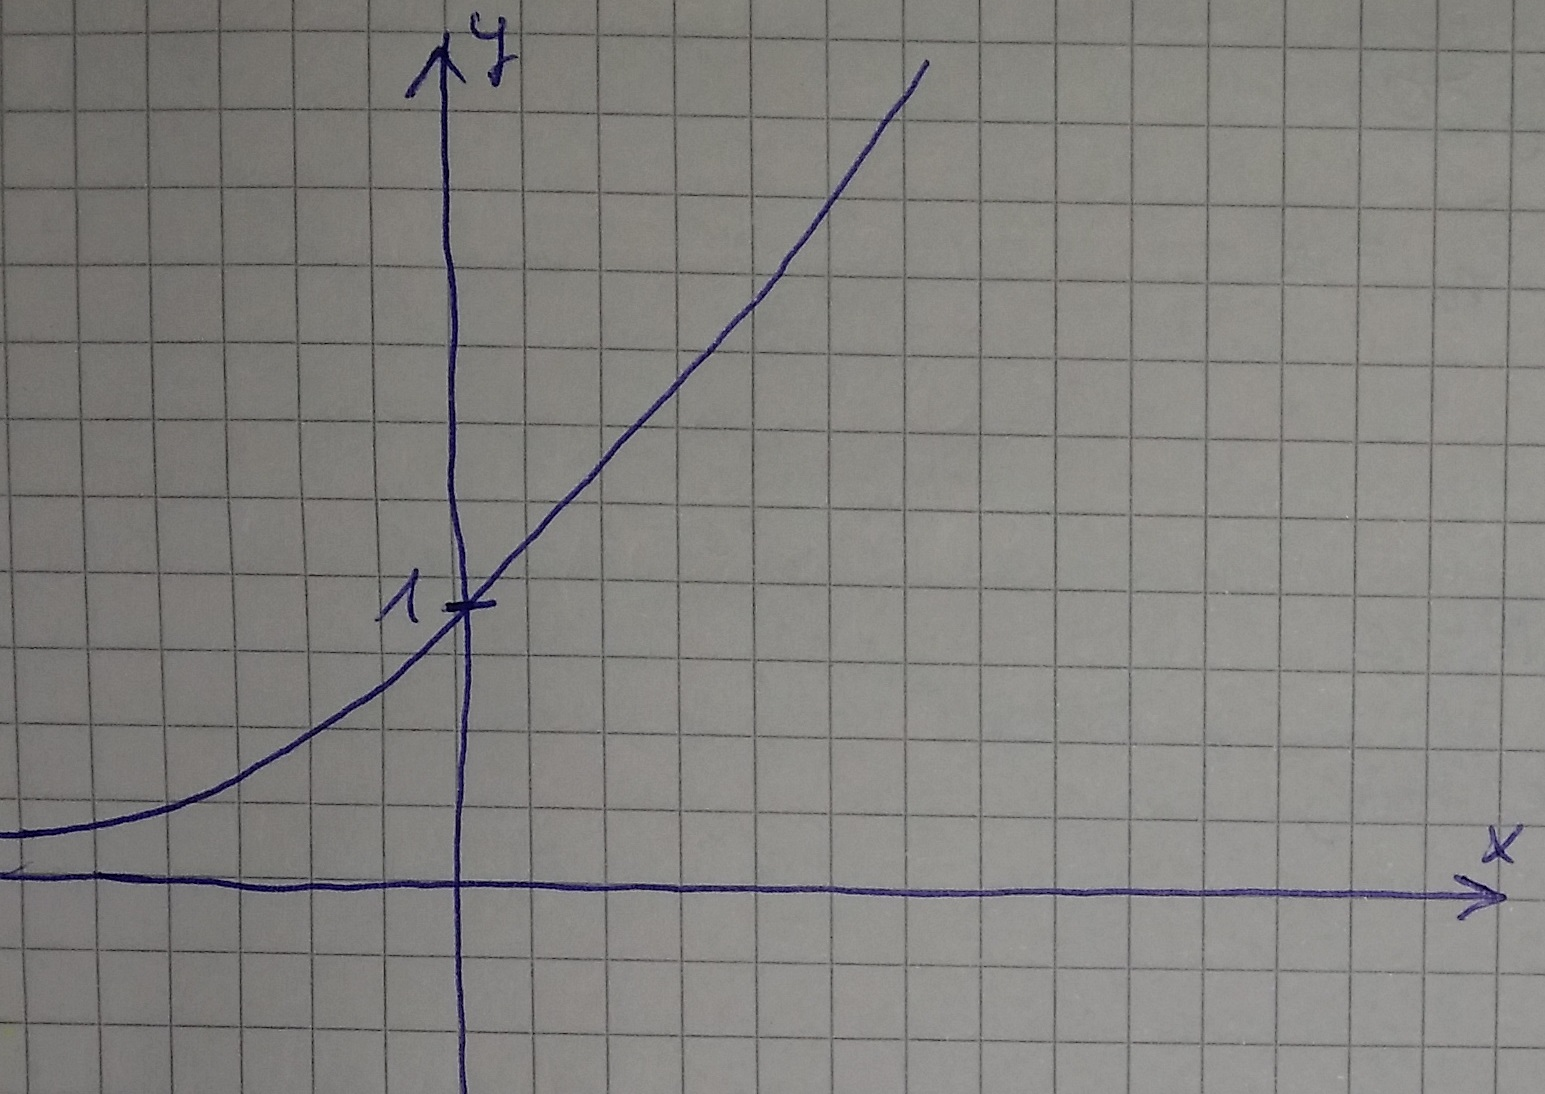
\includegraphics[height=3cm]{kepek/03ea_7.jpg}
		\caption{}\label{}
	\end{figure}
	\begin{definition}
		$\exp$ függvény szigorú monoton növekedő $\R$-en \quad $\Rightarrow \quad \exists$ inverze. 
		
		Jele: \[\ln\quad :=\quad \log\quad :=\quad (\exp)^{-1}\]
		a természetes alapú v. $e$-alapú logaritmus függvény.
	\end{definition}
	\begin{note}
		\begin{enumerate}
			\item $\mathcal{D}_{\ln}=\mathcal{R}_{\exp}=(0,+\infty),\quad \mathcal{R}_{\ln}=\mathcal{D}_{\exp}=\R$.
			
			\begin{figure}[H]
				\centering
				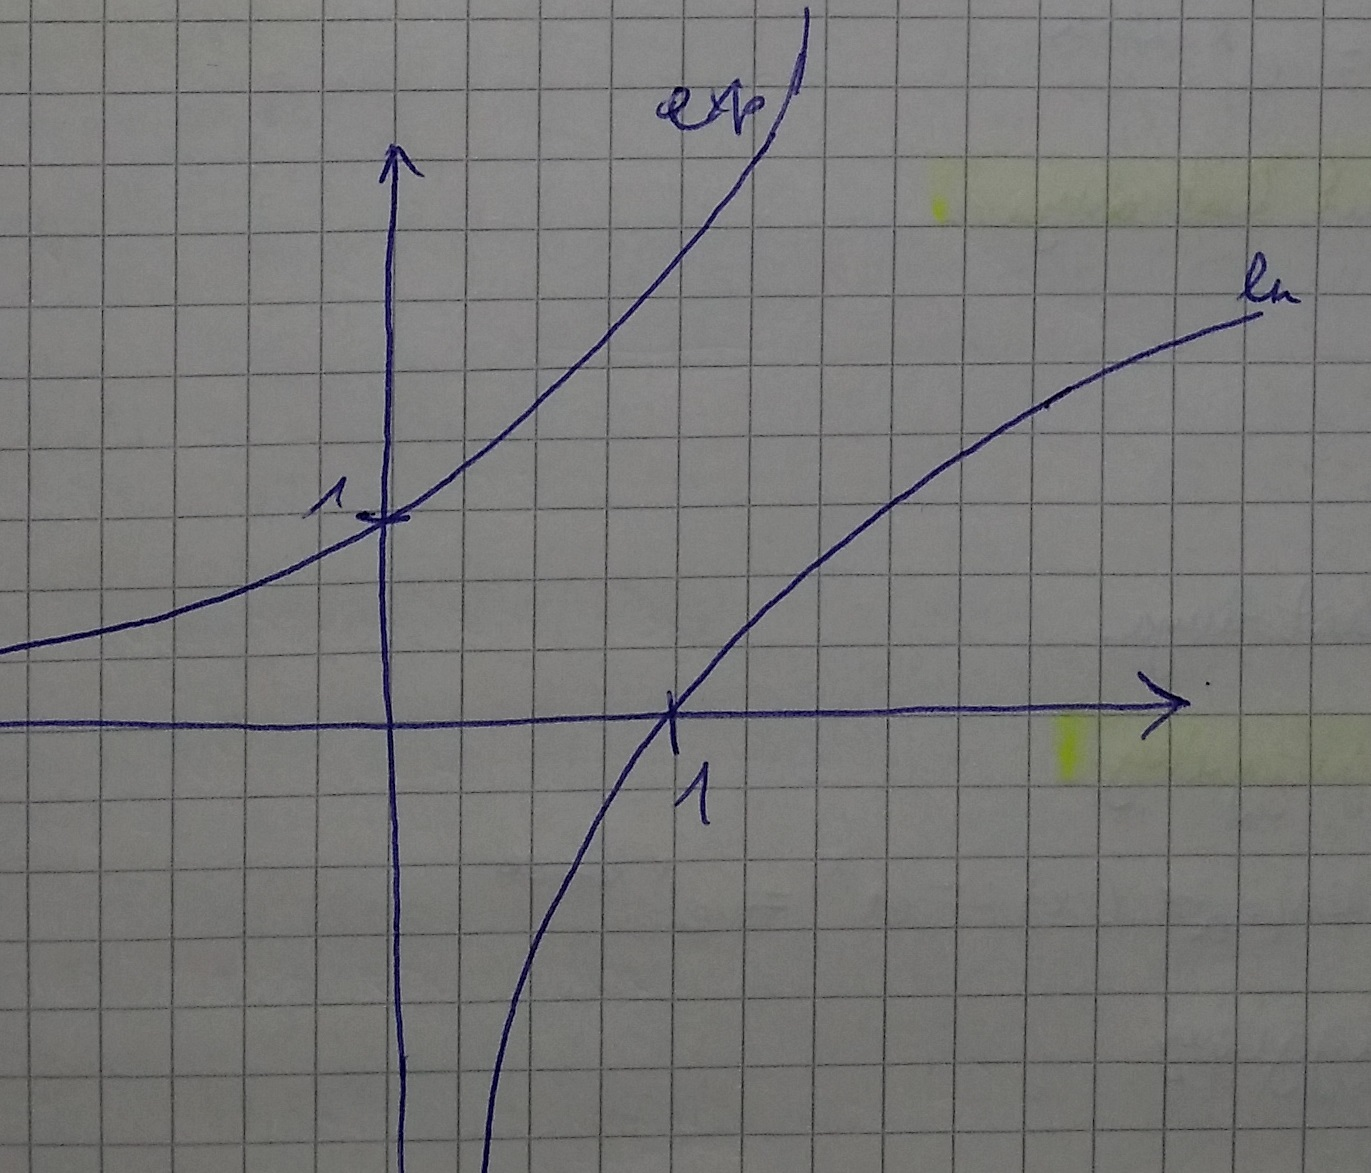
\includegraphics[height=3cm]{kepek/03ea_8.jpg}
				\caption{}\label{}
			\end{figure}
			\item Ha $x>0\quad \Rightarrow\quad \ln x\quad :=\quad \ln(x)\quad :=\quad y \quad \overset{\text{inverz}}{\underset{\text{def.}}{\Rightarrow}}\quad e^y=x$ \quad (lásd: középiskolás definíció)
		\end{enumerate}
	\end{note}
	\begin{theorem}
		(az $\ln$ függvény tulajdonságai)
		\begin{enumerate}
			\item $\ln e^x=x\quad (\forall x \in\R)$\quad  $e^{\ln x}=x\quad (\forall x>0)$
			\item $\ln(xy)=\ln x+\ln y\quad (x,y>0)$
			\item $\ln\uparrow$ és folytonos $(0,+\infty)$-en, $\mathcal{R}_{\ln}=\R$.
			\item $\displaystyle \lim_{0+0}\ln=-\infty; \quad \lim_{+\infty}\ln=+\infty$
		\end{enumerate}
	\end{theorem}
	\begin{note}\ 
		
		\begin{enumerate}
			\item $\exp x$ jól számolható $\forall x\in\R$-re.
			\item $\forall x>0$-ra $\ln x$ értelmezhve van, de így nem számolható.
		\end{enumerate}
	\end{note}
	\subsection{Az $\exp_a$ és $\log_a$ függvények.}
	\begin{note}
		$a>0; \quad x\in\R$, mi legyen $a^x$?
		\begin{itemize}
			\item ha $x\in\Q\checkmark$
			\item ha $x\in\R$ tetszőleges: a hatványazonosságok érvényben maradjanak.
			
			Ötlet: \fbox{$a=e^{\ln a}$}, azaz az $e$-t $a$ hatványként írjuk fel.
			\[ a=e^{\ln a ^x} = e^{x\cdot\ln a} \]
		\end{itemize}
	\end{note}
	\begin{definition}
		$a>0$ valós, $x\in\R$
		\[ a^x:=e^{x\cdot\ln a} \]
		ezt nevezzük az $a$ szám $x$-edik hatványának.
	\end{definition}
	\begin{definition}
		$a>0,\quad \exp_a:\R\to\R,$
		\[ \exp_a(x):=a^x=e^{x\cdot\ln a} \]
		az $a$ alapú exponenciális függvény.
	\end{definition}
	\begin{note}
		$\exp_e=\exp$
		
		Igazolható:
		\begin{itemize}
			\item $0<a\not=1, \quad \exp_a:\R\to(0,+\infty)$ folytonos bijekció.
			\item Ha az $a>1\quad \Rightarrow\quad \exp_a\uparrow,\quad \lim_{-\infty}\exp_a=0,\quad \lim_{+\infty}\exp_a=+\infty$
			\item Ha $0<a<1,\quad $ akkor $\exp\downarrow$,\quad $\lim_{-\infty}\exp_a:=+\infty;\quad \lim_{+\infty}\exp_a=0$
		\end{itemize}
		
		\begin{figure}[H]
			\centering
			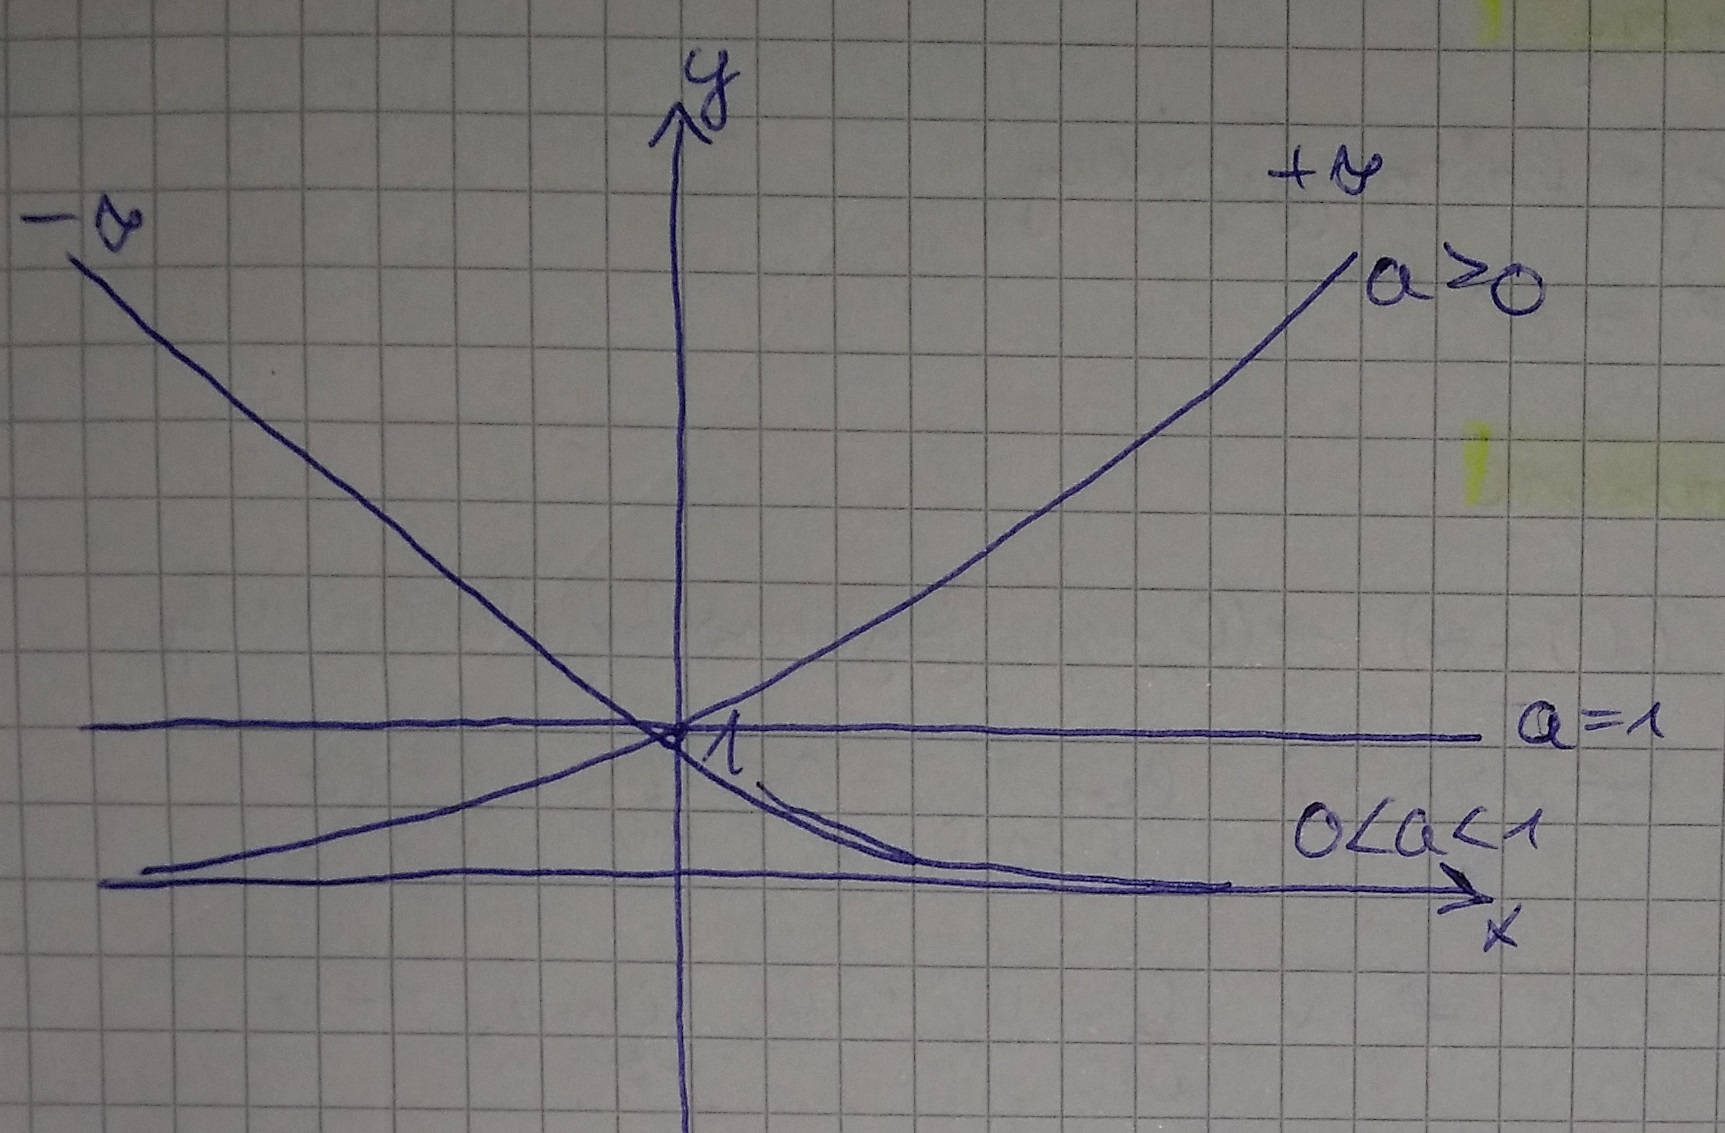
\includegraphics[height=3cm]{kepek/03ea_9.jpg}
			\caption{}\label{}
		\end{figure}
	\end{note}
	\begin{definition}
		$0<a\not=1$ valós$\quad \Rightarrow\quad \exp_a$ szigorúan monoton és folytonos $\R$-en$\quad \Rightarrow\quad \exists$ inverze.
		\[ \log_a:=\left(\exp_a\right)^{-1} \]
		$a$ alapú logaritmus függvény.
	\end{definition}
	\begin{note}
		$\log_e=\ln=\log$
		
		\begin{figure}[H]
			\centering
			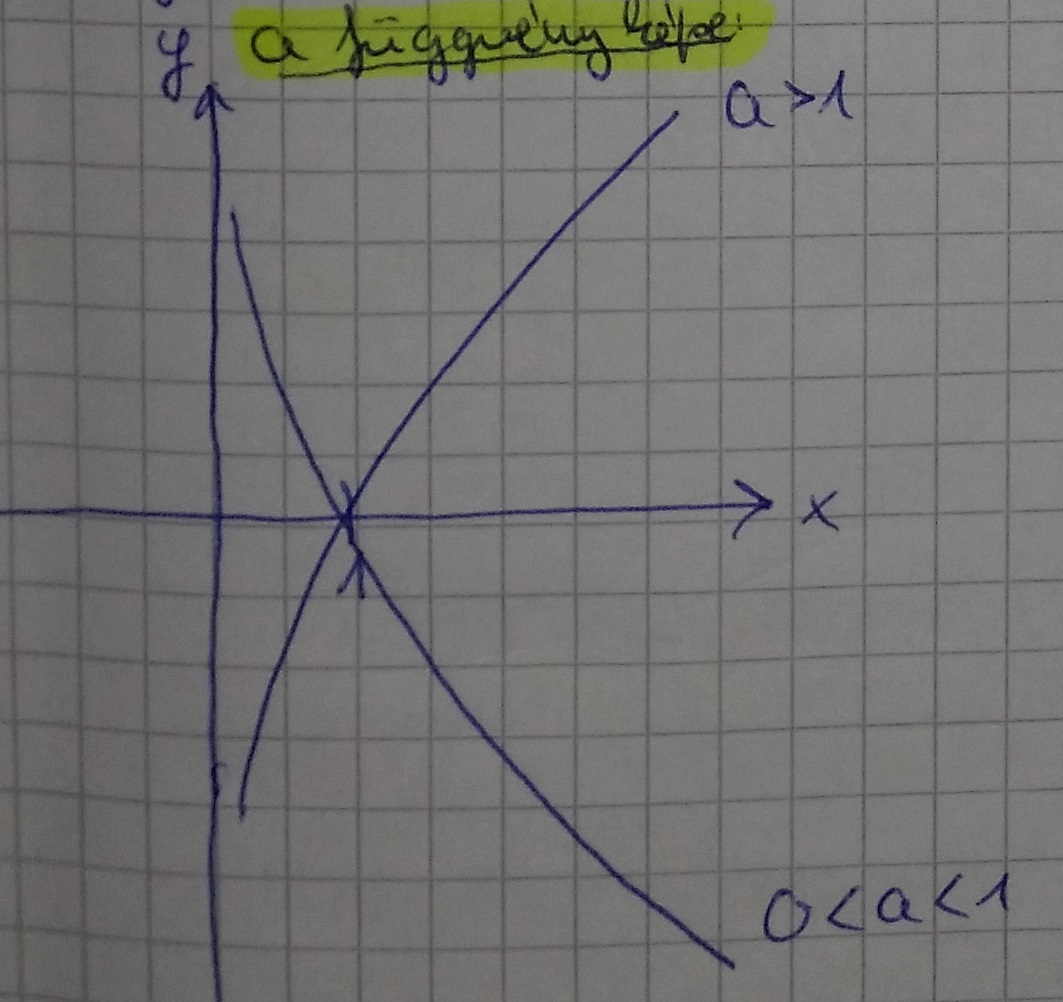
\includegraphics[height=3cm]{kepek/03ea_10.jpg}
			\caption{}\label{}
		\end{figure}
	\end{note}
	\begin{note}
		A függvénytulajdonságok és logaritmusazonosságok megfogalmazhatók (H.F.), megjegyzendők.
	\end{note}
	\subsection{Hatványfüggvények.}
	\begin{definition}
		Legyen $\alpha\in\R$ tetszőleges, \textit{az $\alpha$ kitevőjű hatványfüggvény}:
		\[ h_\alpha:(0,+\infty)\ni x\to x^\alpha=e^{\alpha\cdot\ln x} \]
	\end{definition}
	\begin{theorem}
		(a hatványfüggvény tulajdonságai)
		
		Ha $\alpha\in\R\setminus\{0\} \quad \Rightarrow\quad h_\alpha(0,+\infty)\to(0,+\infty)$ folytonos bijekció, amely 
		\begin{enumerate}
			\item ha $\alpha>0 \quad \uparrow$
			\[ \lim_{0+0} h_\alpha=0,\quad \lim_{+\infty}h_\alpha=+\infty \]
			\item ha $\alpha<0\quad \downarrow$
			\[ \lim_{0+0}h_\alpha=+\infty,\quad \lim_{+\infty}h_\alpha=0 \]
		\end{enumerate}
		
		\begin{figure}[H]
			\centering
			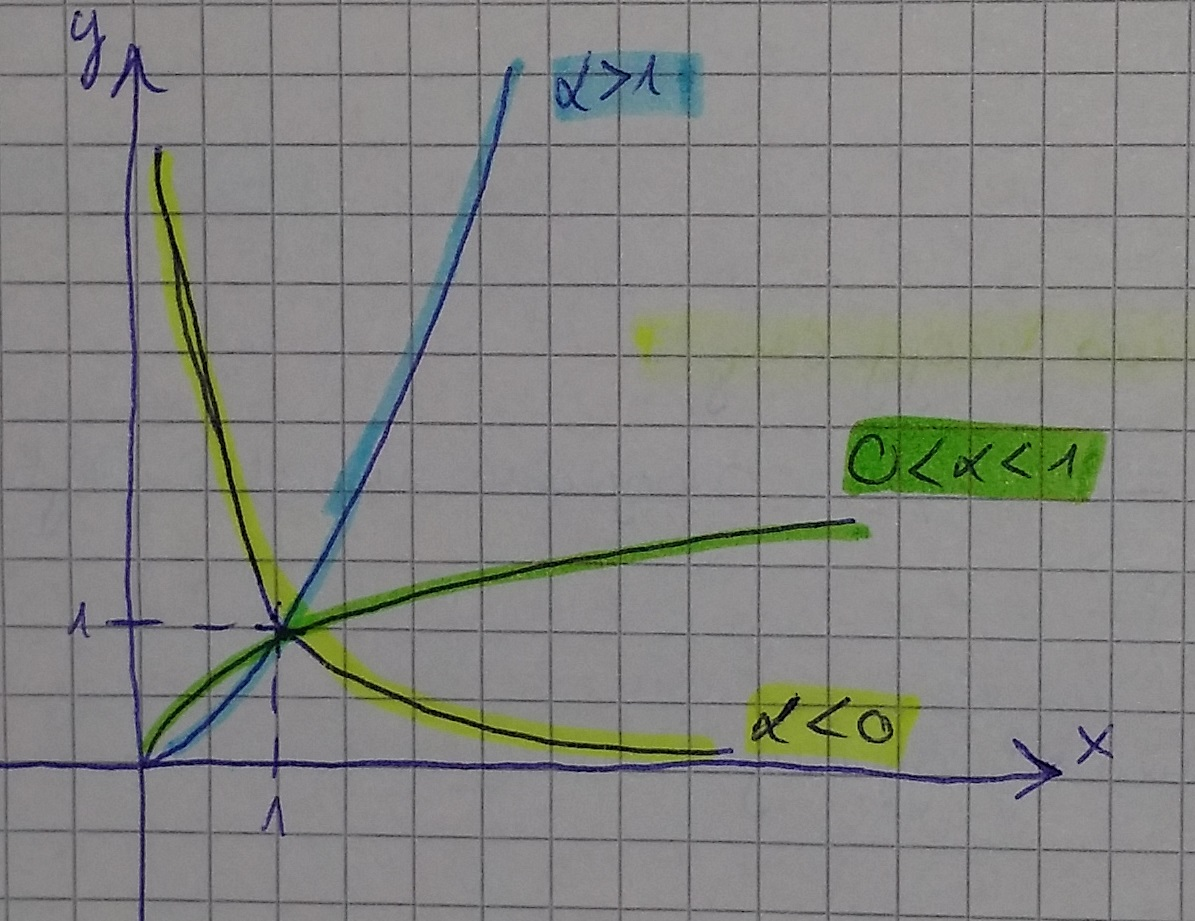
\includegraphics[height=3cm]{kepek/03ea_11.jpg}
			\caption{}\label{}
		\end{figure}
	\end{theorem}
	\section{Differenciálszámítás.}
	\begin{note}
		hóóó crap
	\end{note}
	\begin{revision}
		Határérték (függvénytulajdonság)
	\end{revision}
	A pontbeli derivált motivációja pl. hogy a függvény grafikonjának van-e ,,töréspontja''.
	\begin{figure}[H]
		\centering
		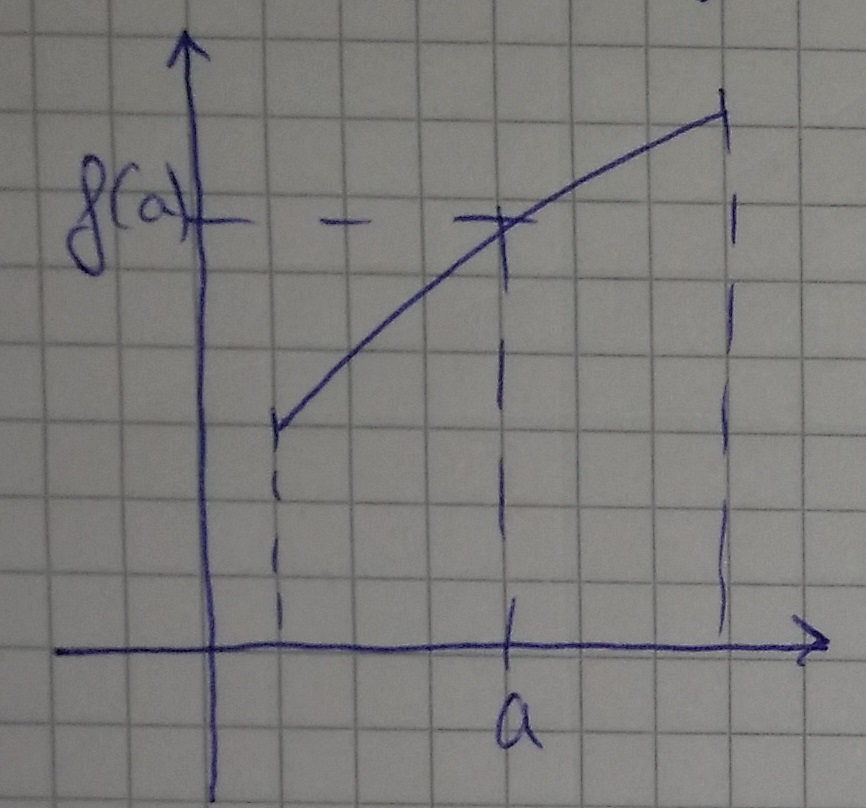
\includegraphics[height=3cm]{kepek/03ea_12a.jpg}\quad \quad \quad 
		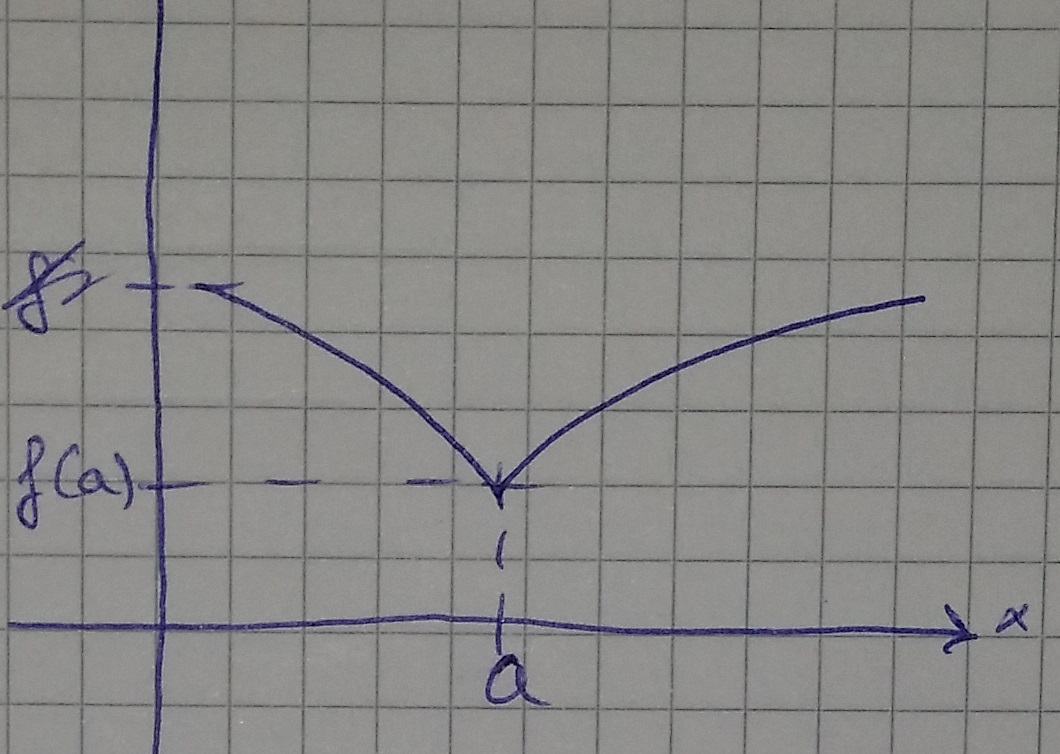
\includegraphics[height=3cm]{kepek/03ea_12b.jpg}
		\caption{Az elsőnek nincs, a másodiknak van töréspontja.}\label{}
	\end{figure}
	Ötlet: $(a,f(a))$-ban szelőt húzni
	\begin{figure}[H]
		\centering
		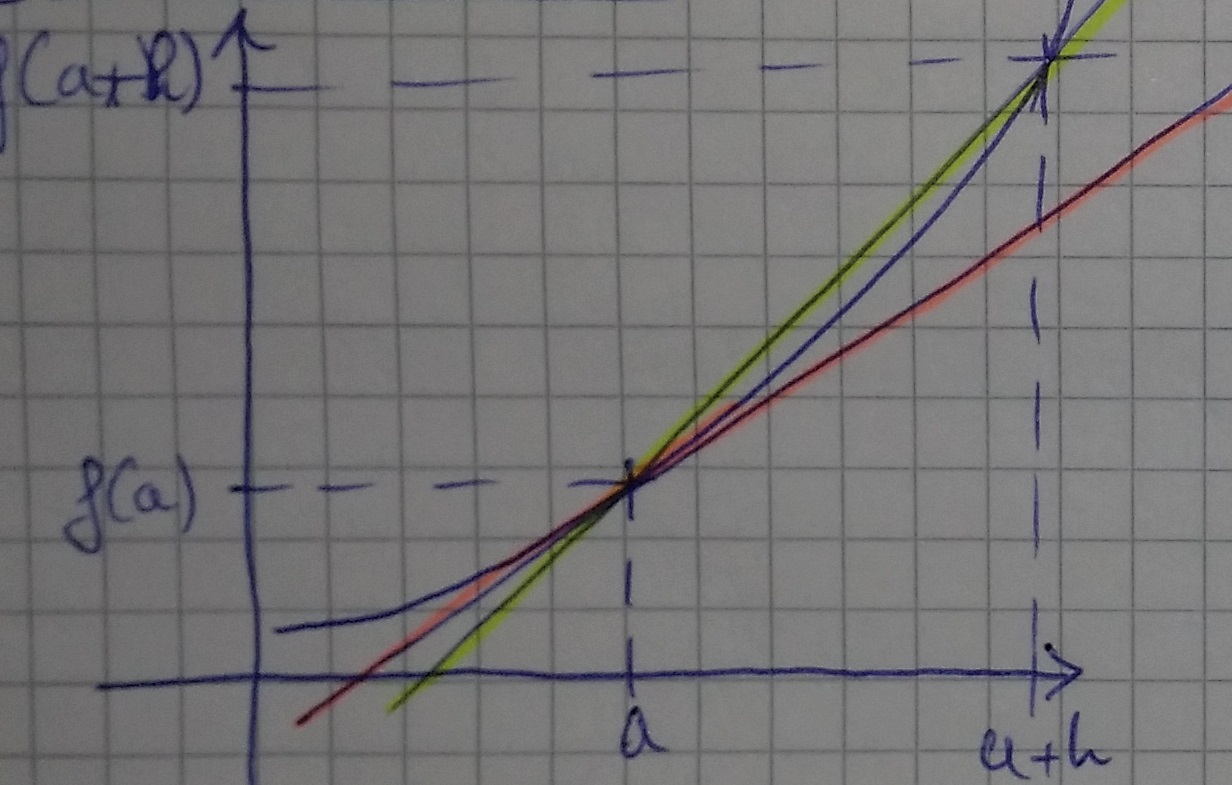
\includegraphics[height=3cm]{kepek/03ea_13.jpg}
		\caption{}\label{}
	\end{figure}
	A szelő meredeksége $m_h=\frac{f(a+h)-f(a)}{h}$ A szelőknek van határhelyzete:
	\[ \exists\lim_{h\to0}\frac{f(a+h)-f(a)}{h} \]
	\begin{figure}[H]
		\centering
		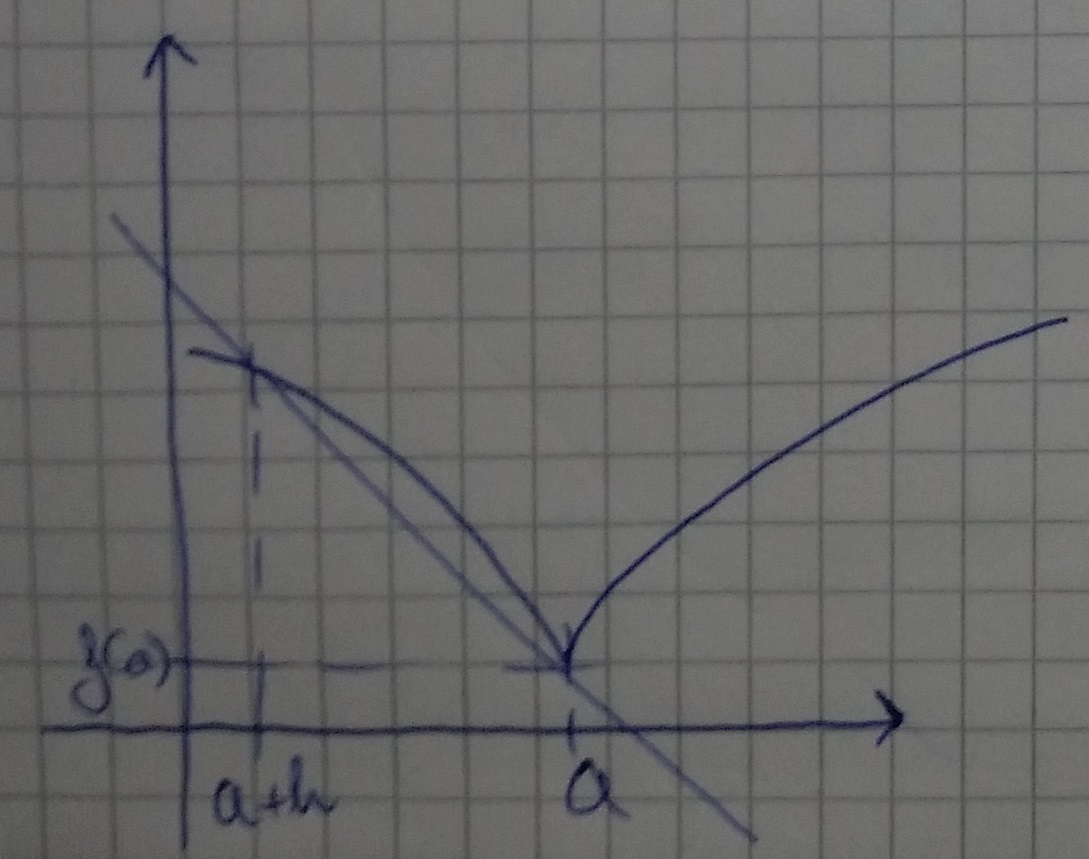
\includegraphics[height=3cm]{kepek/03ea_14.jpg}
		\caption{}\label{}
	\end{figure}
	A szelőknek nincs határhelyzete:
	\[ \nexists\lim_{h\to0}\frac{f(a+h)-f(a)}{h}\quad \blacksquare \]
\end{document}
